% A workaround to allow relative paths in included subfiles
% that are to be compiled separately
% See https://tex.stackexchange.com/questions/153312/subfiles-inside-a-subfile-using-relative-paths
\providecommand{\main}{..}
\documentclass[\main/thesis.tex]{subfiles}
\externaldocument{previous}
\externaldocument{link}

\begin{document}

\chapter{Centrality and Rank}
To rank entities in uncertain networks, as mentioned in Section \ref{CMIUG}, Sevon et al. \cite{sevon2006link} proposed to transform the probabilities into weights by taking the negative logarithm of the probabilities. Pfeiffer and Neville \cite{pfeiffer2010probabilistic} formulated a measure of centrality based on the most probable paths of communication. To facilitate the comparison among our algorithm and these two methods, we rename these two methods Negative Logarithm (NL) and Most Likely Path (ML).

\section{Inversed Probabilistic Graph} \label{Inversed-Probabilistic-Graph}

A major shortcoming of both NL and ML methods is that they can only be applied to unweighted probabilistic graphs. For a weighted probabilistic graph, ignoring the original weights of the graph could cause the two methods to perform badly, which we will show later in the experiment part. In order to solve this problem, we propose a new approach, Inversed Probabilistic Graph (IPG), defined as follow:

In Section \ref{Uncertain-Network-Definition}, we define the uncertain network as $\mathcal{G = (V,E,P)}$, which can be regarded as the definition of an unweighted uncertain network. In this Chapter, as we aim to solve the problem of entity ranking in both unweighted and weighted networks, we redefine the uncertain network as $\mathcal{G = (V,E,P,W)}$, where $\mathcal{V}$ is the collection of vertices, $\mathcal{E}$ the collection of edges, $\mathcal{P}$ is the probability distribution over the edges and $\mathcal{W}$ is the collection of original weights over the edges. For an arbitrary edge $e \in \mathcal{E}$, we divide the original weight by the corresponding edge probability to a power of $\lambda$,
\begin{equation}
w'(e) = \frac{w(e)}{p(e)^\lambda }. \label{ipg}
\end{equation}
In this way, the probabilistic graph $\mathcal{G}$ becomes the inversed probabilistic graph $IPG = (V, E, W)$ where $W$ contains the adjusted edge weights that are computed from Equation \ref{ipg}.

Now similar to NL, we can apply standard shortest path algorithms used in deterministic graphs to the IPG, and betweenness and closeness centralities can be calculated accordingly. The intuition behind it is that the less distance between two nodes in the graph, the larger probability two nodes still have link, hence the closer relationship two nodes should have. The adjusted weight can be calculated in $O(|E|)$, then we can calculate shortest paths for the IPG in $O(|V||E|+|V|^2 \log|V|)$ by running Dijkstra algorithm. The $\lambda$ here is a tunable hyper-parameter. For sake of generosity, all experiments (except Section \ref{Hyper-Parameter-Validation}) described later use $\lambda = 0.4$. 

It's worth noting that:
\begin{enumerate}
%\begin{itemize}
\item Unweighted probabilistic graph is a special case of weighted probabilistic graph: Compared to previously discussed two methods, we expand the applicability of our IPG method to weighted graphs. Actually an unweighted probabilistic graph can be regarded as a special case of weighted probabilistic graph. For weighted uncertain networks, $w(e)$ in Equation \ref{ipg} can be replaced with 1.
\item Deterministic graph is a special case of probabilistic graph: Probability depicts our confidence/knowledge of the existence of an edge. If we are sure that an edge $e_{uv}$ exists, then $p(e_{uv}) = 1$ and $w'(e_{uv}) = \frac{w(e_{uv})}{p(e_{uv})^\lambda } = w(e_{uv})$, meaning that in this case the adjusted weight is exactly the original weight of the graph. Conversely, if an $e_{uv}$ is believed to be non-existent for certain, then $p(e_{uv}) = 0$ and $w'(e_{uv}) = \frac{w(e_{uv})}{p(e_{uv})^\lambda } = \infty$, indicating that the distance between nodes $u$ and $v$ is infinitely large, i.e., there is no interaction between these two nodes in the graph.
\end{enumerate}
%\end{itemize}

\section{Experiment}
\subsection{Betweenness Centrality Ranking Evolution}
To investigate the performance of our proposed IPG method, we first conduct an illustrative experiment as Pfeiffer \cite{pfeiffer2010probabilistic,pfeiffer2011methods} did. We use the same method as section 5 in \cite{pfeiffer2010probabilistic} to assign each edge with a possibility of occurrence. We also perform our experiment on the same dataset as in \cite{pfeiffer2010probabilistic,pfeiffer2011methods}, which is a subset of Enron, comprised of emails sent between employees, resulting in a dataset with 50,572 emails among 151 employees. We pick two pairs of employees in the dataset, visualizing the evolution of betweenness centrality rankings (BCR) for each pair respectively. 
\begin{figure}
\centering
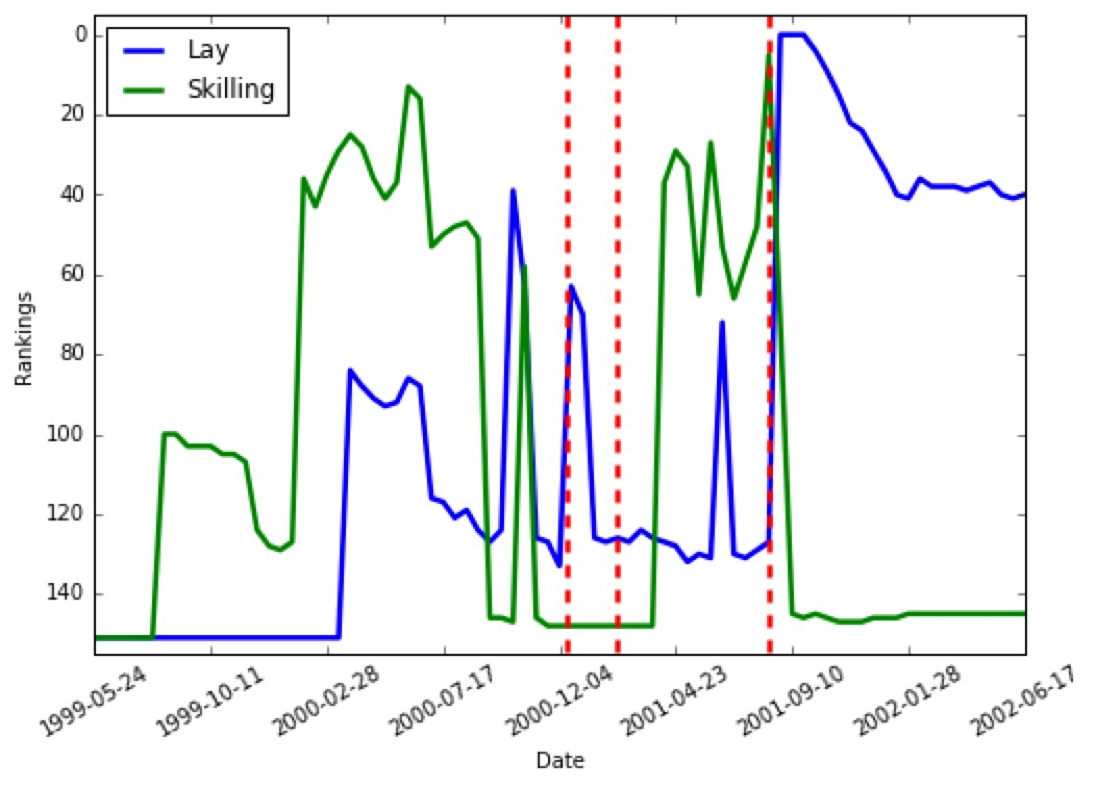
\includegraphics[scale = 0.45]{\main/img/rank_change1.png}
\caption{Betweenness centrality ranking evolution of Lay and Skilling}
\label{rank_change1}
\end{figure}
\subsection*{Lay and Skilling}
First, we analyze two key figures at Enron: Kenneth Lay and Jeffrey Skilling, whose centrality ranking evolutions are shown in Figure \ref{rank_change1}. The background is that Lay was the CEO of the company first, then he handed it over to Skilling. Several months later, Skilling resigned as CEO, relinquishing control back to Lay. We analyze the change of their centrality rankings during the transition periods. We expect that the trends in the figure can reflect what really happened at that period of time.

The first vertical red line in Figure \ref{rank_change1} marks the time $\textit{Dec. $13^{th}$}$ $\textit{2000}$, when it was announced that Skilling would assume the CEO position at Enron, with Lay retiring but remaining as a chairman. In Figure \ref{rank_change1}, our IPG approach identifies a spike in BCR for both Lay and Skilling. This can be naturally explained as Skilling and Lay should be informing other executives about the transition right before it was about to be announced. The second event is during \textit{February, 2001} (marked by the second vertical red line), when Skilling made the official transition to CEO. We can see in the figure that the BCR of Skilling has a steep increase afterwards. Whereas during that period, the BCR of Lay dropped significantly. Seven months later, on \textit{Aug. $14^{th}$, 2001}, Skilling resigned as CEO and Lay took over again. Hence it is no surprise in Figure \ref{rank_change1} near the third vertical red line, that Lay's BCR rose to a high level again and Skilling's went down. 

Moreover, the overall trends of BCR evolution correspond to the real development of the two people. For example, during Skilling's tenure as CEO, he remained a quite high level of centrality ranking; We also notice that the Lay's BCR is higher in the transition period than that during his tenure as CEO. This indicates that a secretary or someone was handling the generic communications with other people for Lay, while during eventful time like job transition, he would communicate with others directly; The third observation is that during the gap between Lay's first and second tenure as CEO, he still kept a certain level of centrality, which can be explained by the fact that he remained as a chairman during his retirement.

\begin{figure}
\centering
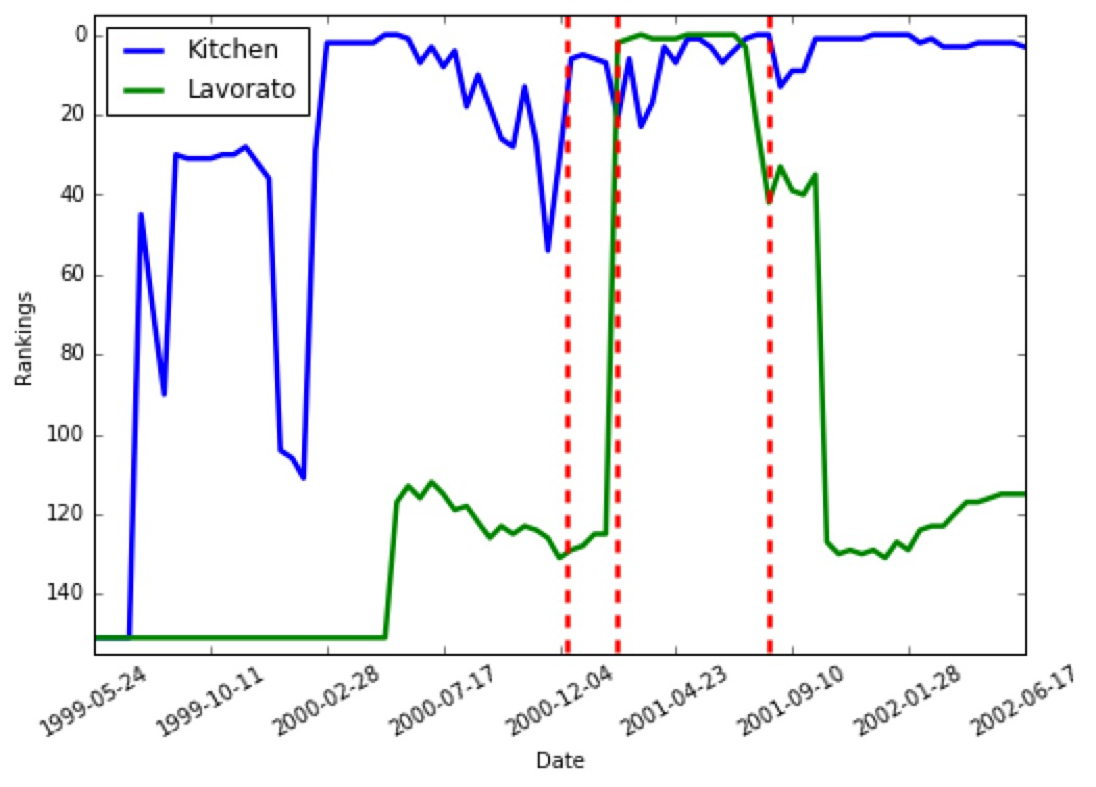
\includegraphics[scale = 0.45]{\main/img/rank_change2.png}
\caption{Betweenness centrality ranking evolution of Kitchen and Lavorato}
\label{rank_change2}
\end{figure}

\subsection*{Kitchen and Lavorato}
The second pair of individuals that we are interested in is Louise Kitchen and John Lavorato, who were executives for Enron America. We can see in Figure \ref{rank_change2} BCR of Kitchen and Lavorato. The first salient discovery is that Lavorato's ranking is extremely high only during Skilling's tenure as CEO. His ranking drops noticeably otherwise. In comparison, Kitchen keeps a relatively high ranking overtime. This indicates that Lavorato has a close relationship with Skilling, whereas Kitchen could have been playing a key role at Enron throughout the time scope.

\subsection{Linear Correlations} \label{Linear-Correlations}
To consolidate the correctness of our method, we also compare our IPG method against NL and ML. We carry out the comparative experiments on Enron dataset, synthetic unweighted graph, and synthetic weighted graph, respectively. The way we evaluate each method is to visualize the linear relationship between centrality rankings computed by each method and the average centrality rankings computed by sampling. Since all the three datasets are either dynamic network or generated dataset, the ground truth of entity rankings is not available in these datasets. However, the Law of Large Numbers shows that, the more samples, the closer the estimation is to the expectation. Therefore, we contend that in the case where there is no ground truth, a strong linear correlation with sampling can be a reasonable indicator of a good method. 

So, let $\mathcal{G}$ be the given probabilistic graph, with probabilistic distribution $\mathcal{P}$ over the edges, we sample $N$ discrete, deterministic graphs $G_1, G_2, ..., G_N$ from $\mathcal{G}$. (In Section \ref{Linear-Correlations} and Section \ref{Hyper-Parameter-Validation}, we choose $N=500$.) We use $CR_{i}(G_{j})$ to denote the centrality ranking of a given node $\mathcal{V}_i$ on a given discrete, (un)weighted graph $G_{j}$. For a given node $\mathcal{V}_i$, the expected centrality ranking of that node in $\mathcal{G}$ is:
\begin{equation}
\mathbb{E}(CR_{i}(\mathcal{G})) = \frac{\sum_{j=1}^{N}CR_{i}(G_j)}{N}
\end{equation}
After calculating the expected centrality ranking for each node, we rank all the nodes in $\mathcal{G}$ again according to their expected ranking values. We refer to this newly computed ranking as \textit{overall ranking}. As of experiments, we apply each target method to probabilistic graph $\mathcal{G}$ to get the overall rankings for all nodes in $\mathcal{G}$. We visualize the result by drawing a 2D plot of overall rankings of nodes computed by each target method against the average rankings of nodes computed from sampling. 
\begin{equation}
r = \frac{\sum_{i=1}^{m} |x_i - y_i|}{\sqrt{2}m} \label{linear}
\end{equation}
We use Equation \ref{linear} as the metric of the linear relationship strength, where $m$ is the number of total nodes in $\mathcal{G}$, $i$ indexes of the target node and ($x_i, y_i$) is the coordinates of the $i^{th}$ node in the plot. Hence $x_i$ is  the average centrality ranking of $N$ sampled graphs, and $y_i$ is the overall ranking computed by a certain method.

\begin{figure}
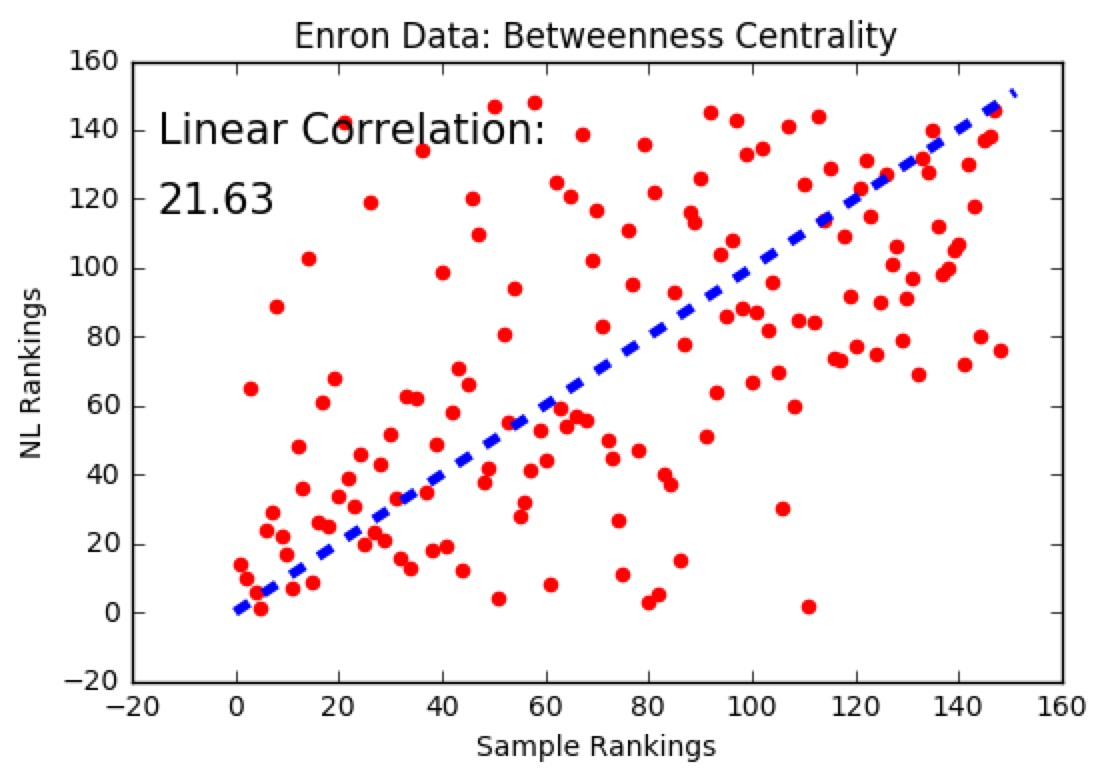
\includegraphics[scale = 0.17]{\main/img/EBC_NL.jpeg}
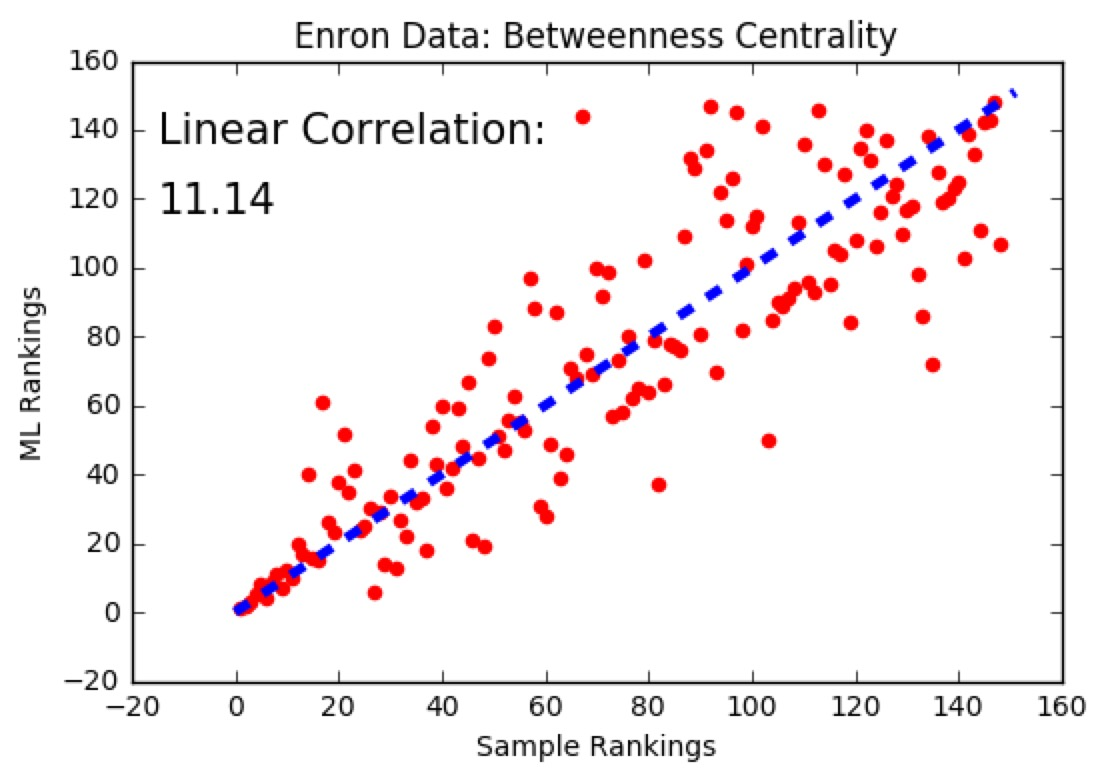
\includegraphics[scale = 0.17]{\main/img/EBC_ML.jpeg}
\centering
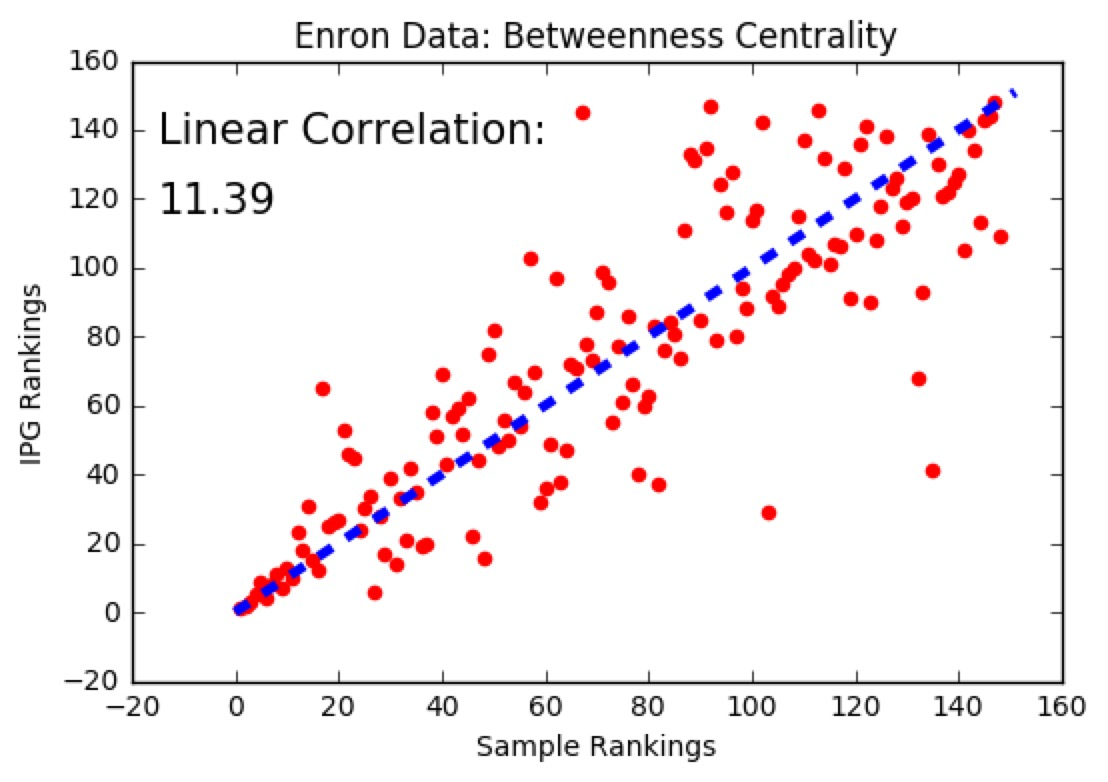
\includegraphics[scale = 0.17]{\main/img/EBC_IPG.jpeg}

\caption{Betweenness centralities computed by different methods on Enron dataset}
\label{btw_enron}
\end{figure}

\begin{figure}
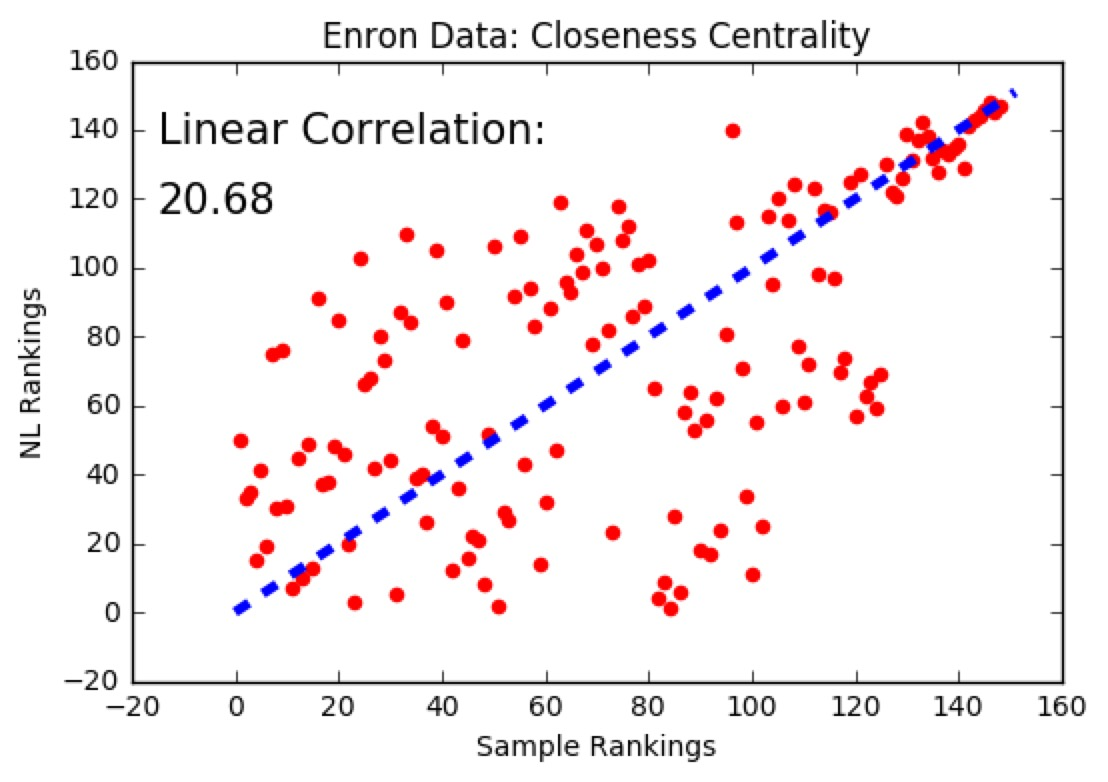
\includegraphics[scale = 0.17]{\main/img/ECC_NL.jpeg}
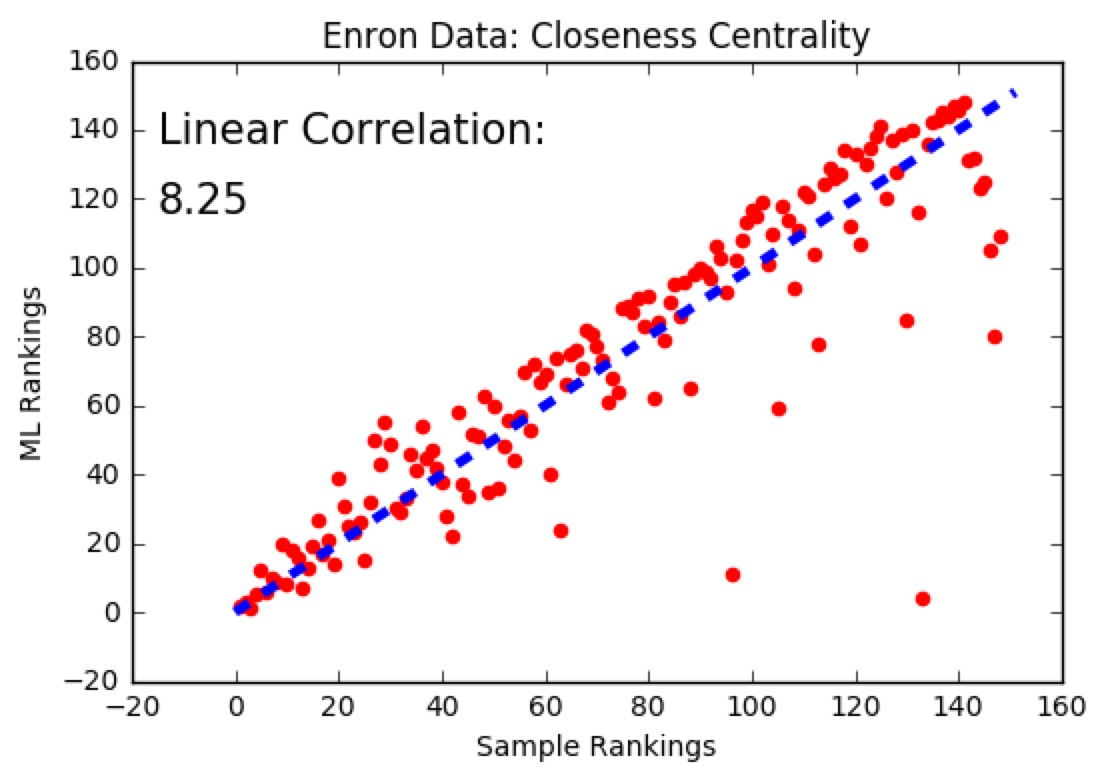
\includegraphics[scale = 0.17]{\main/img/ECC_ML.jpeg}
\centering
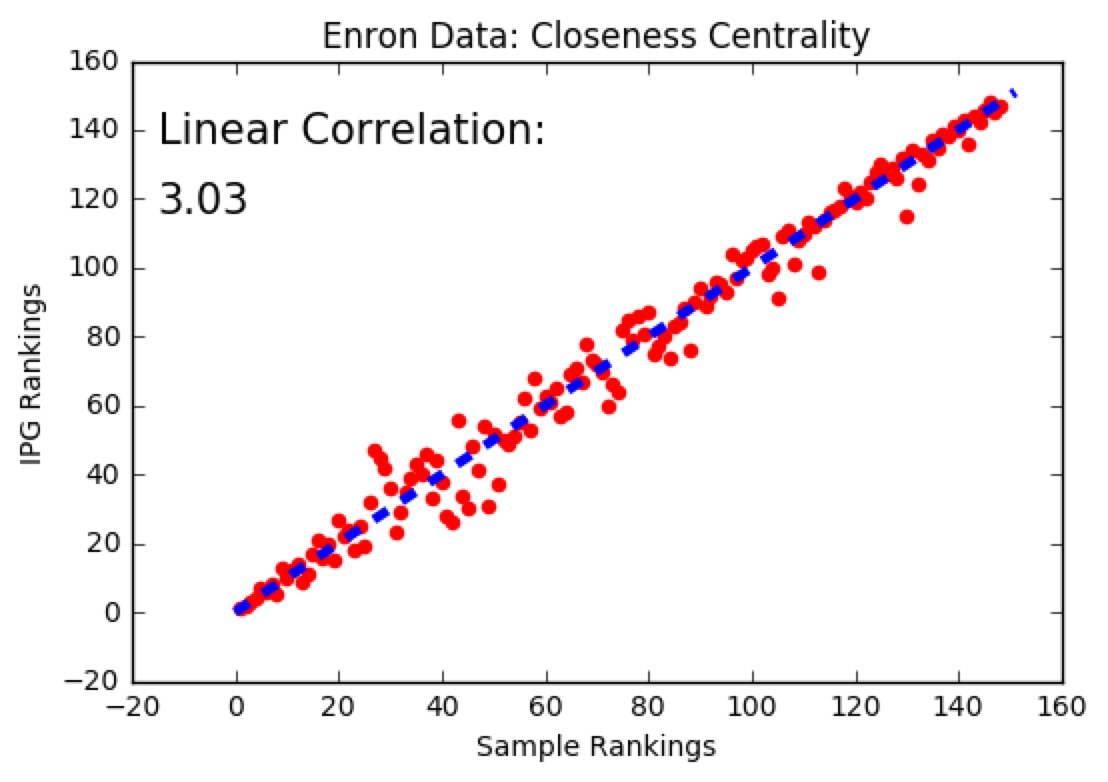
\includegraphics[scale = 0.17]{\main/img/ECC_IPG.jpeg}
\caption{Closeness centralities computed by different methods on Enron dataset}
\label{cl_enron}
\end{figure}


\subsubsection{Enron Dataset}
Figure \ref{btw_enron} shows the betweenness centrality rankings on Enron dataset computed by NL, ML, and IPG respectively, at a particular point in time: November $14^{th}$, 2001. The linear correlation values are displayed on the plots as well. We can easily tell that our IPG method outperforms the NL method, and is slightly worse than ML method.

Figure \ref{cl_enron} is the same experiment as Figure \ref{btw_enron} except that we compute closeness rather than betweenness. In terms of closeness centrality on the same dataset, IPG can outperform both NL and ML.

\begin{figure}
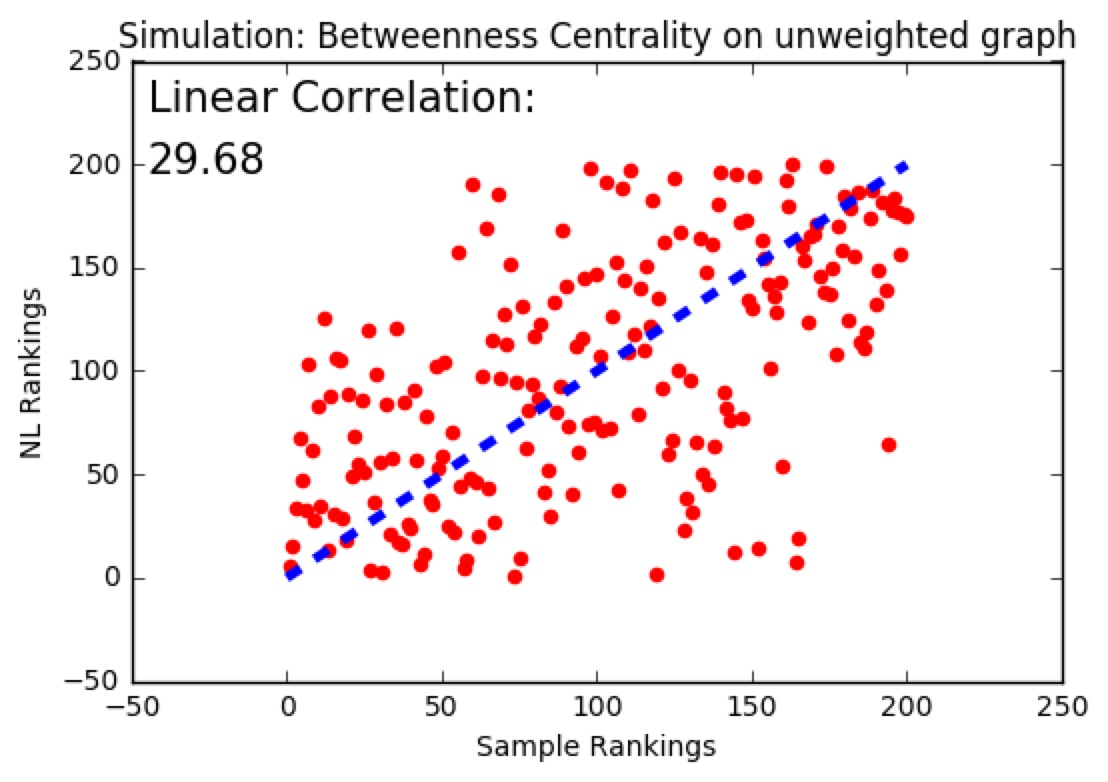
\includegraphics[scale = 0.17]{\main/img/BCU_NL.jpeg}
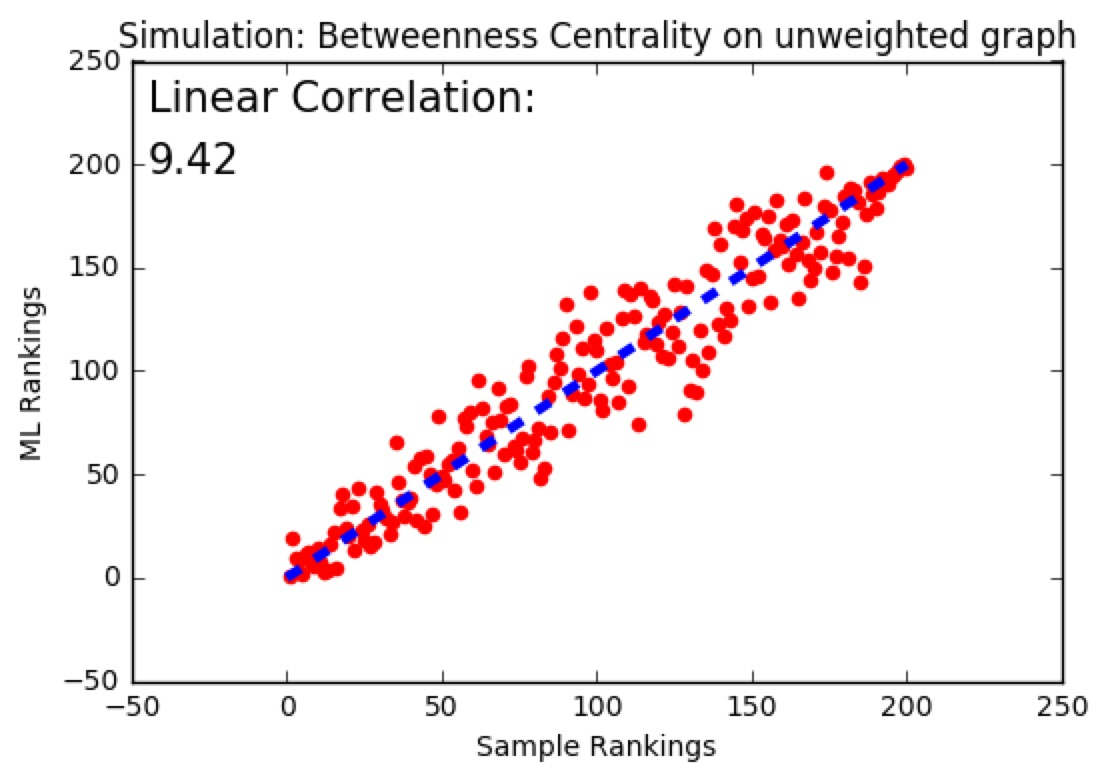
\includegraphics[scale = 0.17]{\main/img/BCU_ML.jpeg}
\centering
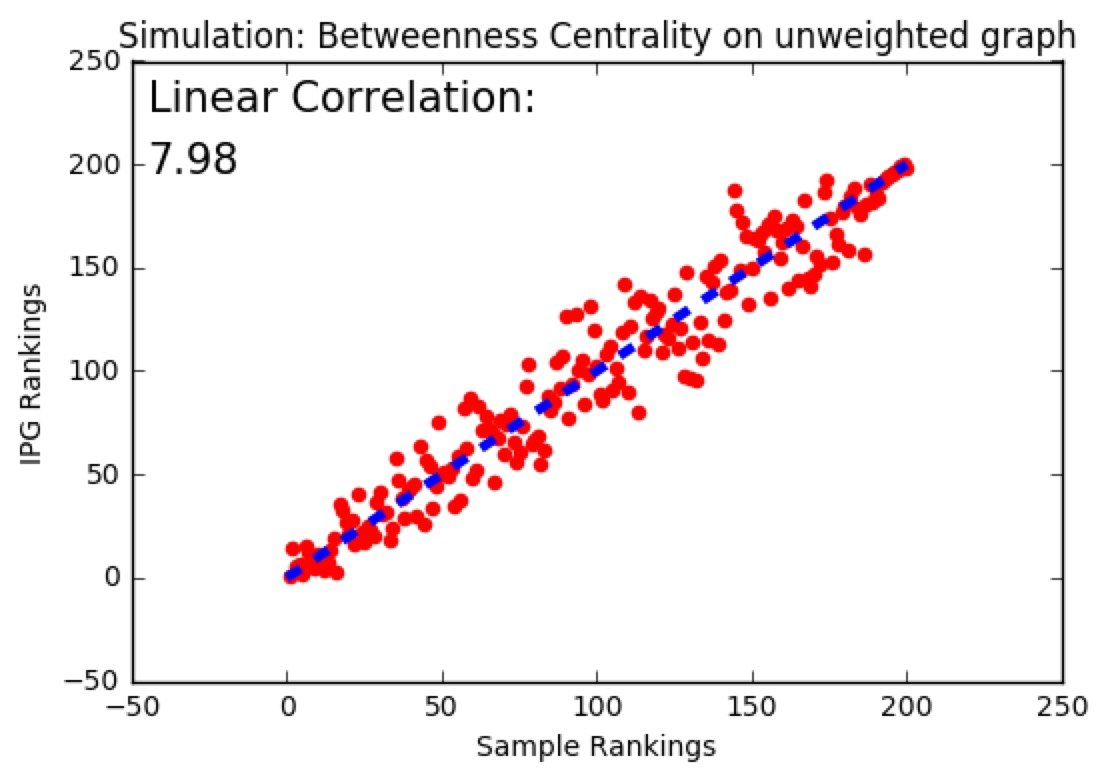
\includegraphics[scale = 0.17]{\main/img/BCU_IPG.jpeg}
\caption{Betweenness centralities computed by different methods on synthetic unweighted graphs}
\label{btw_unweighted}
\end{figure}

\begin{figure}
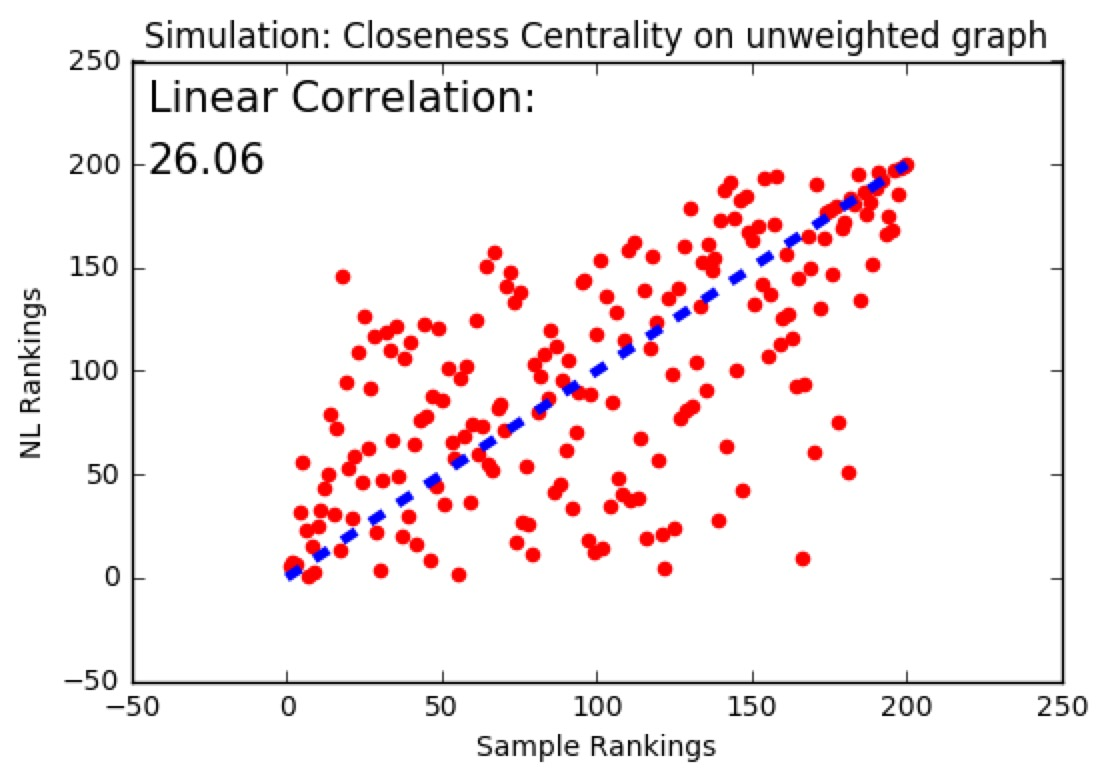
\includegraphics[scale = 0.17]{\main/img/CCU_NL.jpeg}
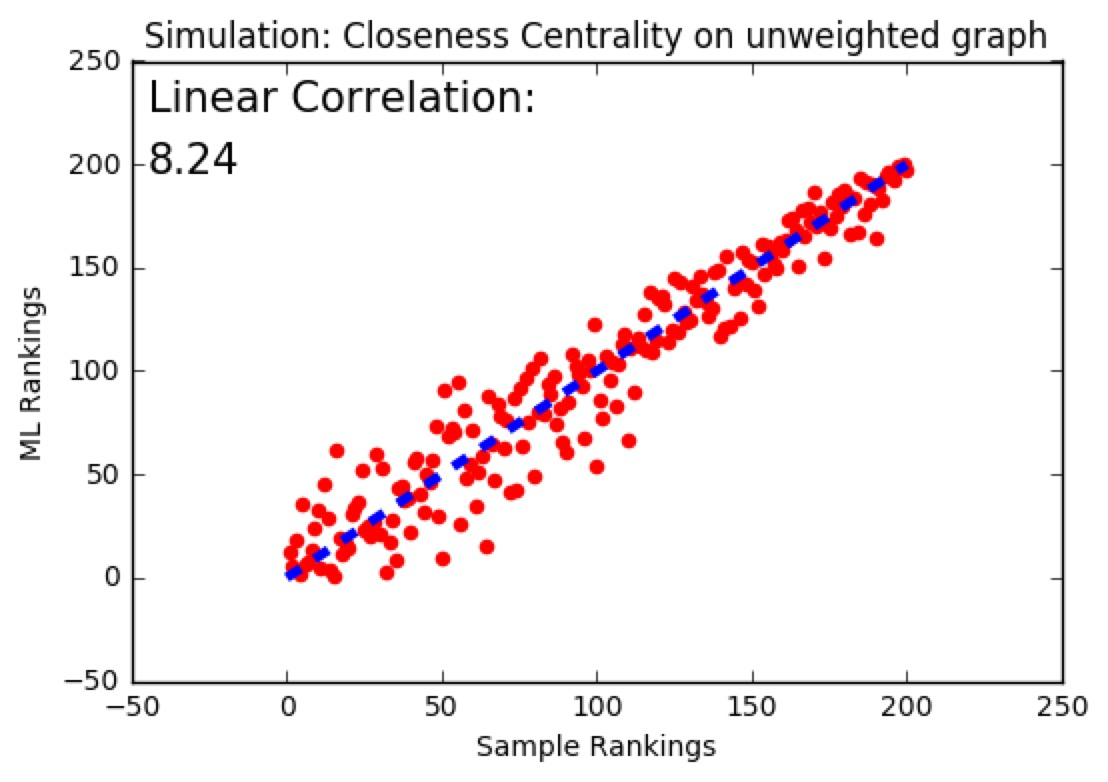
\includegraphics[scale = 0.17]{\main/img/CCU_ML.jpeg}
\centering
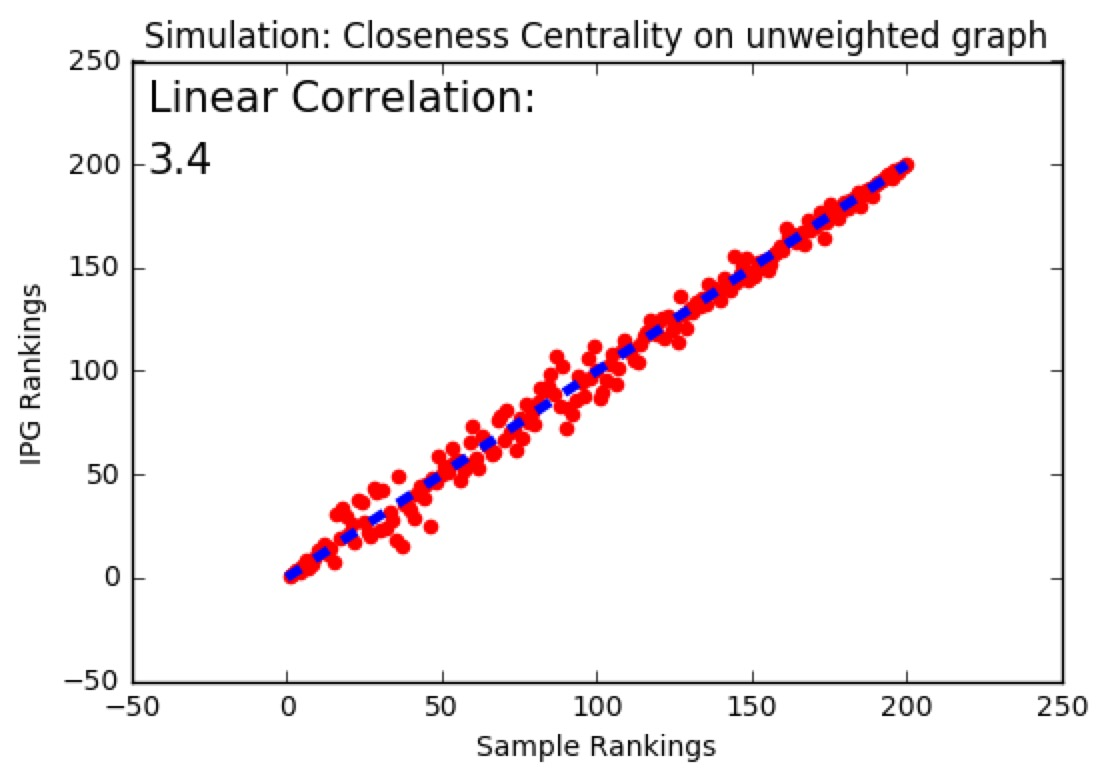
\includegraphics[scale = 0.17]{\main/img/CCU_IPG.jpeg}
\caption{Closeness centralities computed by different methods on synthetic unweighted graphs}
\label{cl_unweighted}
\end{figure}

\subsubsection{Unweighted Graphs} \label{Unweighted-Graphs-Experiment}
We also implement experiment on synthetic unweighted graphs. We generate three communities with the number of nodes in each community being 30, 50, and 120, respectively. The probability of \textit{within-community} connection is 0.2, and the probability of \textit{between-community} connection is 0.02. Then we use uncertain network generator (Algorithm \ref{Uncertain-Network-Generator} as mentioned in Section \ref{Synthetic-Uncertain-Network-Based-on-Deterministic-Network}) to generate an uncertain network based on the given certain network. 

The betweenness centrality results of three methods are displayed in Figure \ref{btw_unweighted} and the closeness results are in Figure \ref{cl_unweighted}. For all three methods, the linear correlation in closeness experiment are stronger than that in betweenness experiment. But no matter in which case, our IPG always exhibits the best performance among the three and NL has the worst performance.

\subsubsection{Weighted Graphs}
We pointed out earlier that one major advantage of IPG over NL and ML is that our method extends well on weighted graphs. We show this advantage in this section via experiment. The experimental parameters are inherited from the former Unweighted Graphs experiment, and the weights assigned to edges are generated based on a uniform distribution on the interval $[1,3]$. Figure \ref{btw_weighted} and Figure \ref{cl_weighted} respectively show the betweenness and closeness of three methods on weighted graphs. As the plots in two figures indicate, IPG still has the best performance among the three methods in terms of both betweenness and closeness centrality rankings.

\begin{figure}
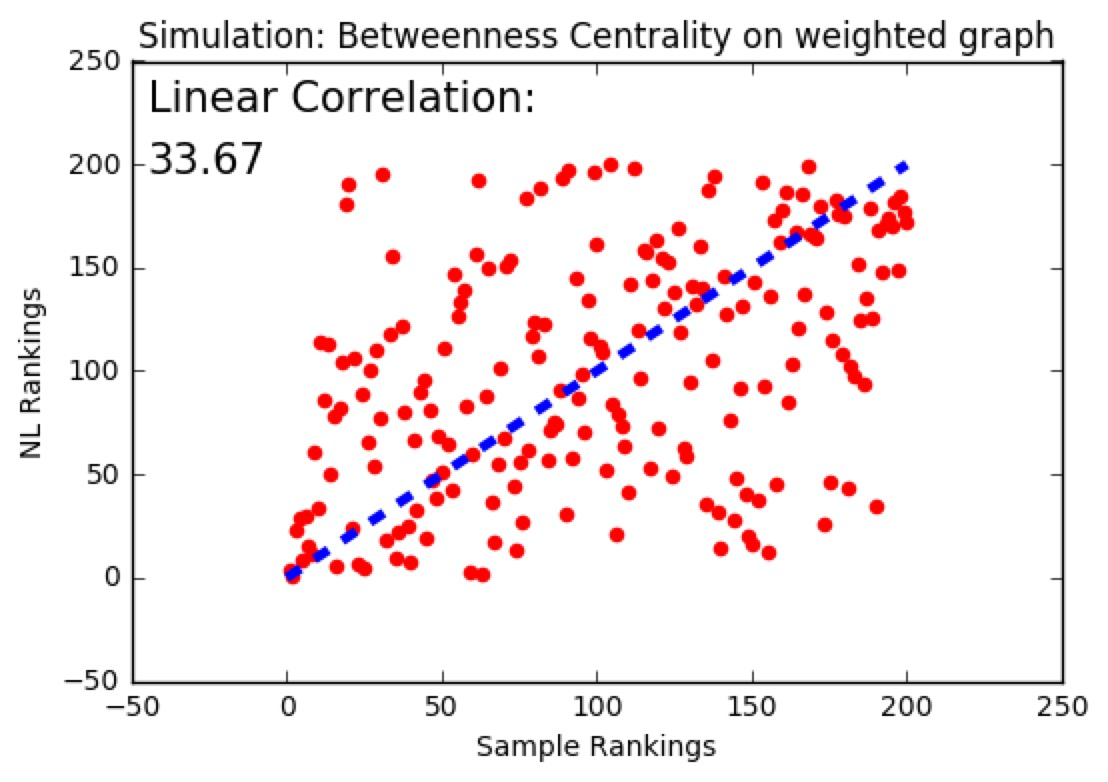
\includegraphics[scale = 0.17]{\main/img/BCW_NL.jpeg}
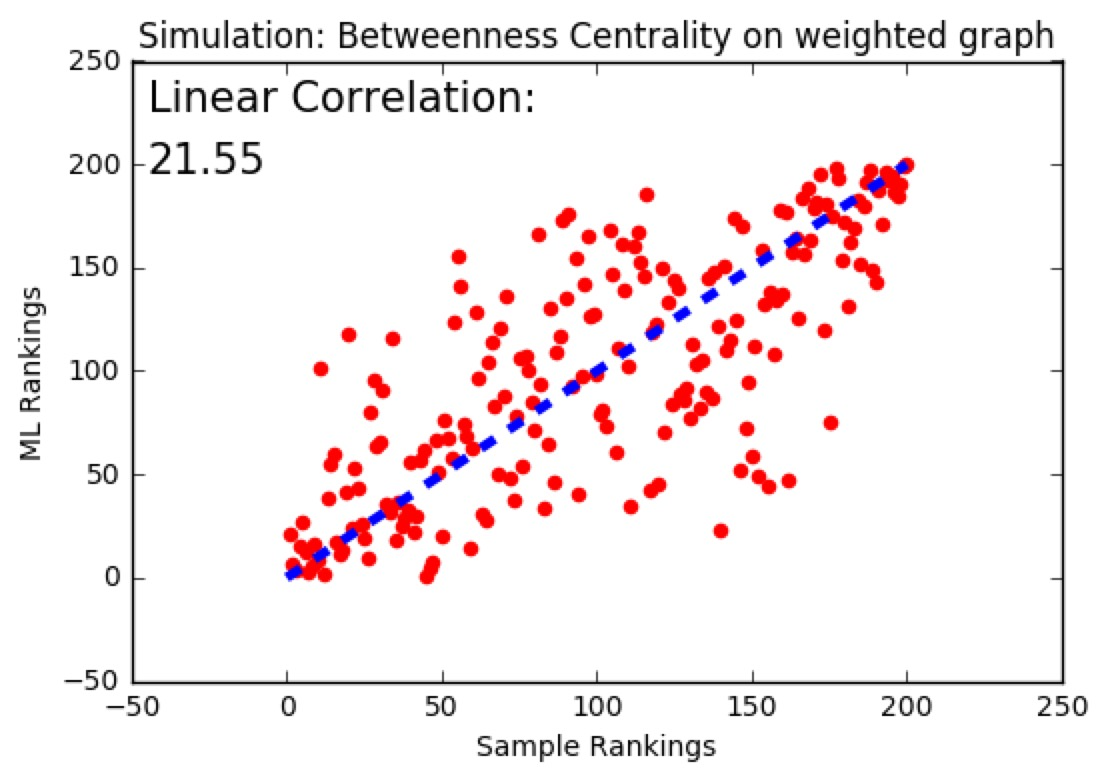
\includegraphics[scale = 0.17]{\main/img/BCW_ML.jpeg}
\centering
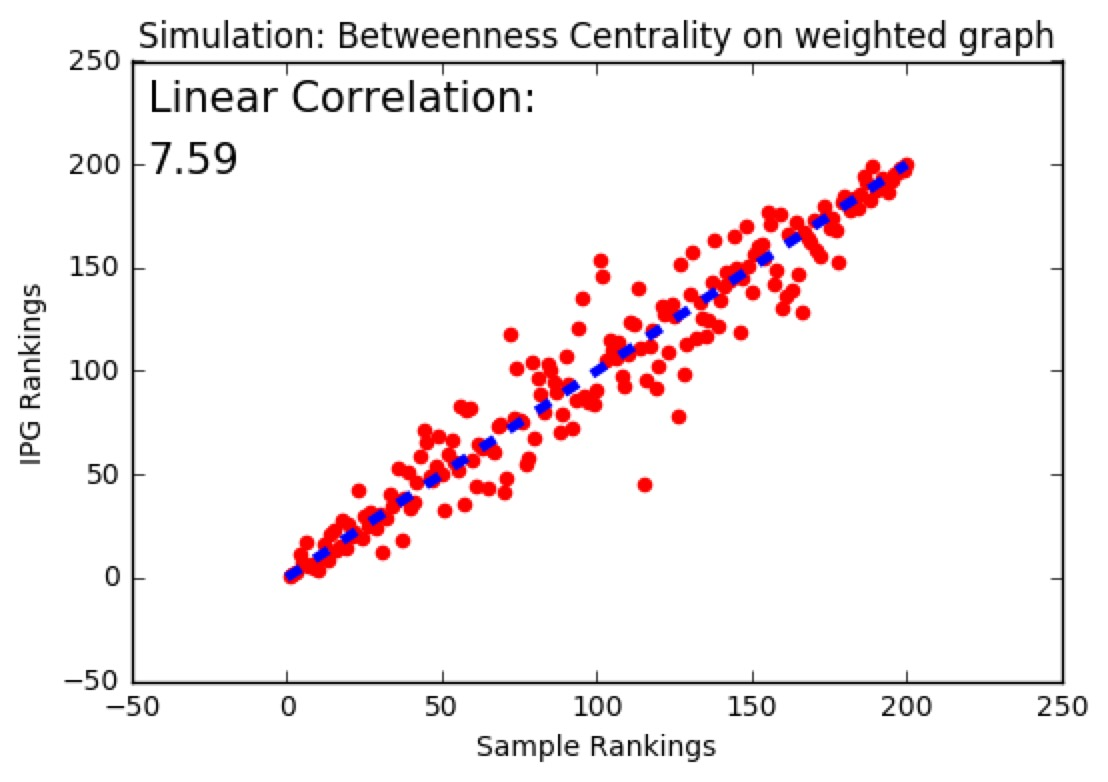
\includegraphics[scale = 0.17]{\main/img/BCW_IPG.jpeg}
\caption{Betweenness centralities computed by different methods on synthetic weighted graphs}
\label{btw_weighted}
\end{figure}


\begin{figure}
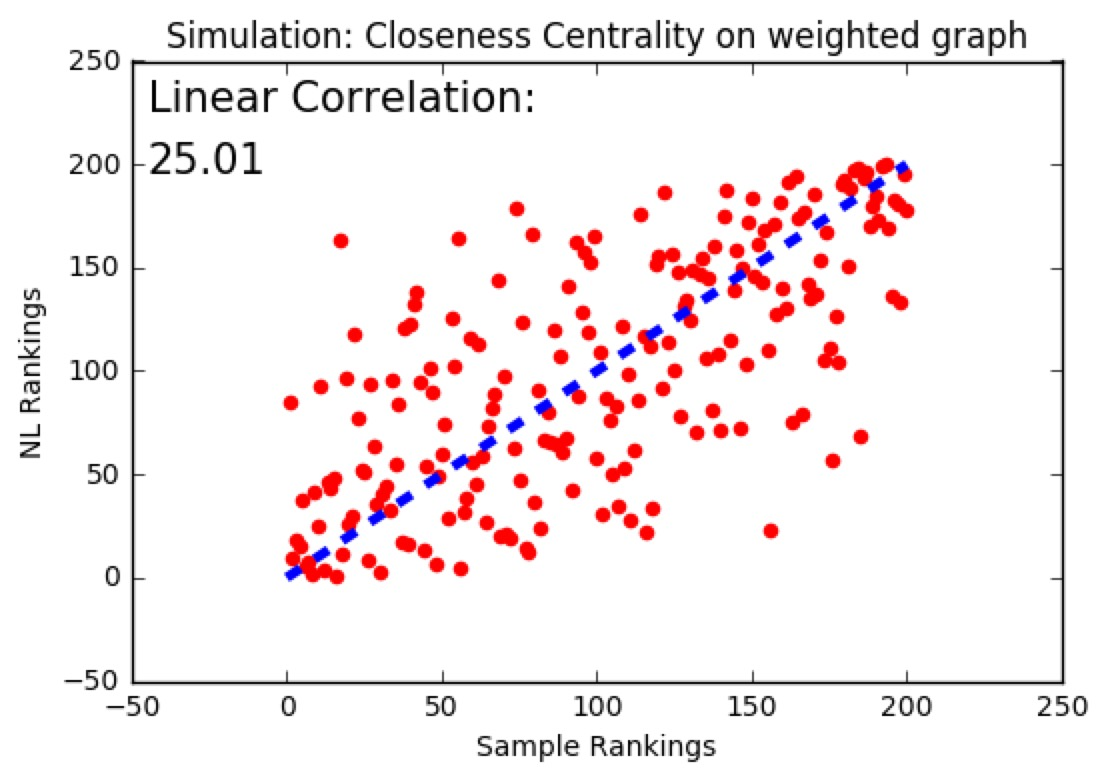
\includegraphics[scale = 0.17]{\main/img/CCW_NL.jpeg}
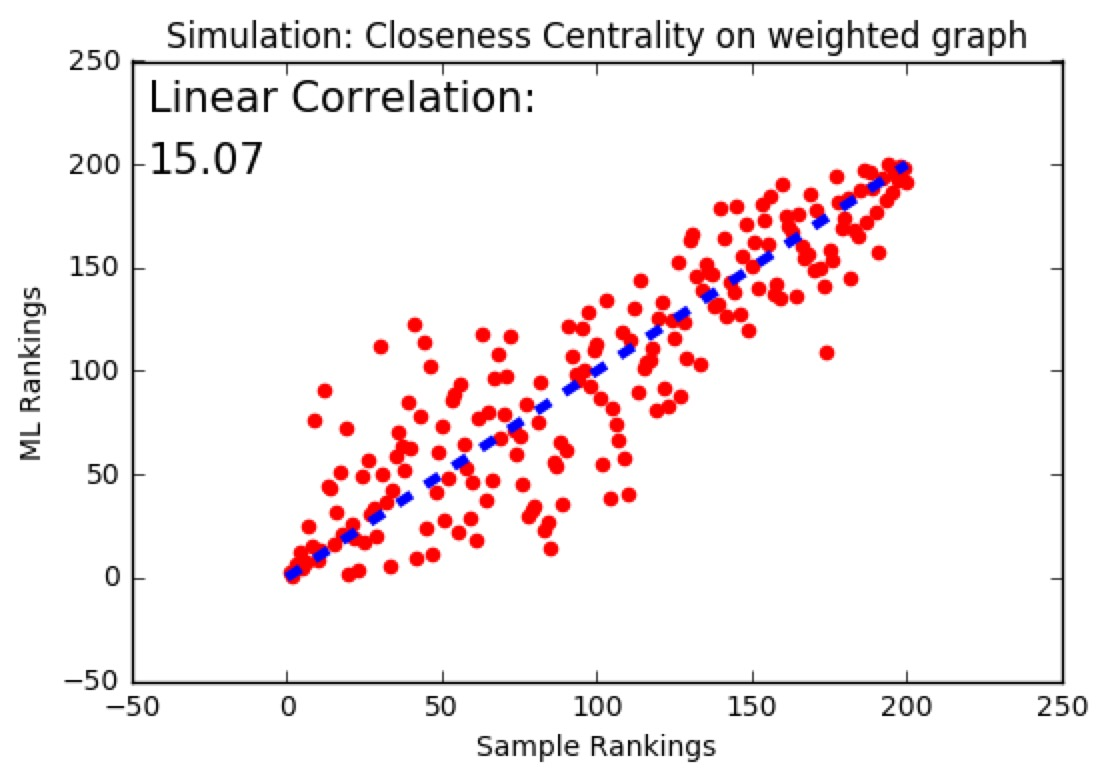
\includegraphics[scale = 0.17]{\main/img/CCW_ML.jpeg}
\centering
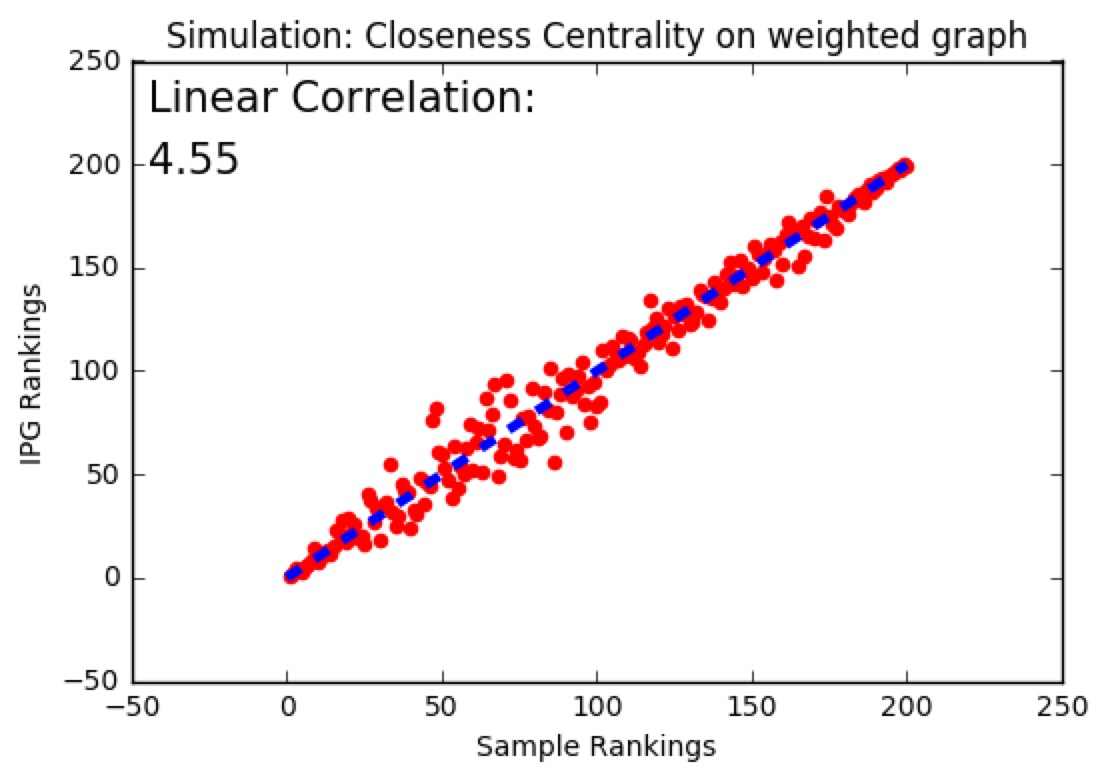
\includegraphics[scale = 0.17]{\main/img/CCW_IPG.jpeg}
\caption{Closeness centralities computed by different methods on synthetic weighted graphs}
\label{cl_weighted}
\end{figure}


\subsection{Hyper-parameter Validation} \label{Hyper-Parameter-Validation}
As we mentioned in Section \ref{Inversed-Probabilistic-Graph}, the choice of hyper-parameter $\lambda$ is another crucial topic in our experiment. To validate that the $\lambda$ value we use is a reasonable choice, we conduct experiments in this section to find optimal $\lambda$ for different centrality measures on different graphs. We do this by repeating previous experiments on synthetic unweighted and weighted graphs over a range of different $\lambda$ values, as shown in Figure \ref{hyper}.

\begin{figure}
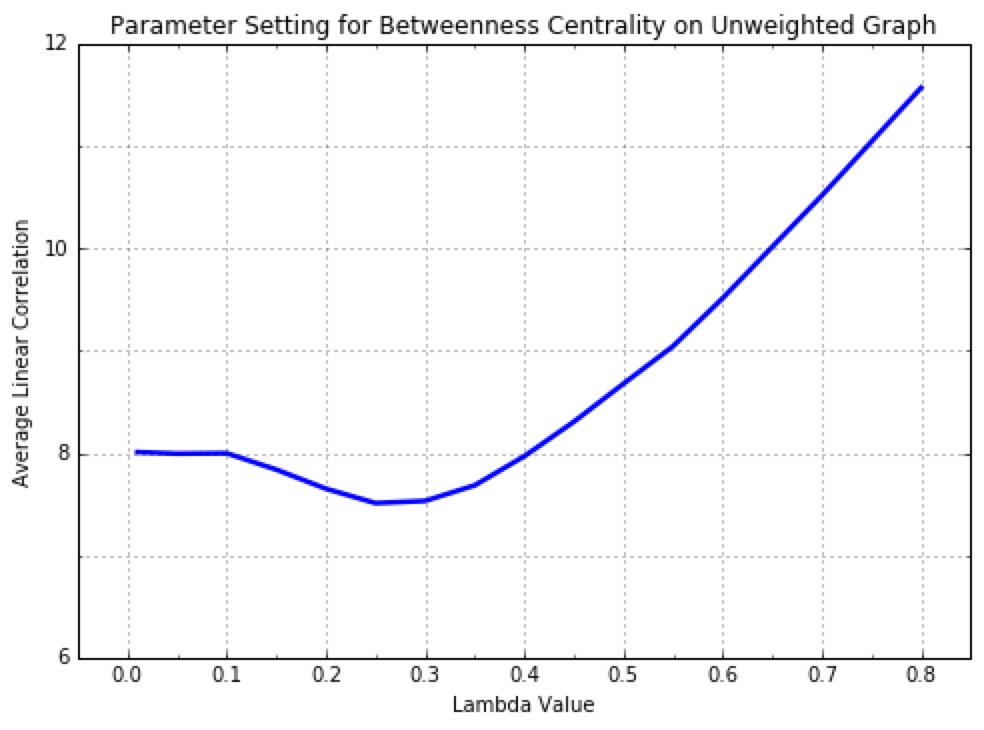
\includegraphics[scale = 0.2]{\main/img/BCU_2.jpeg}
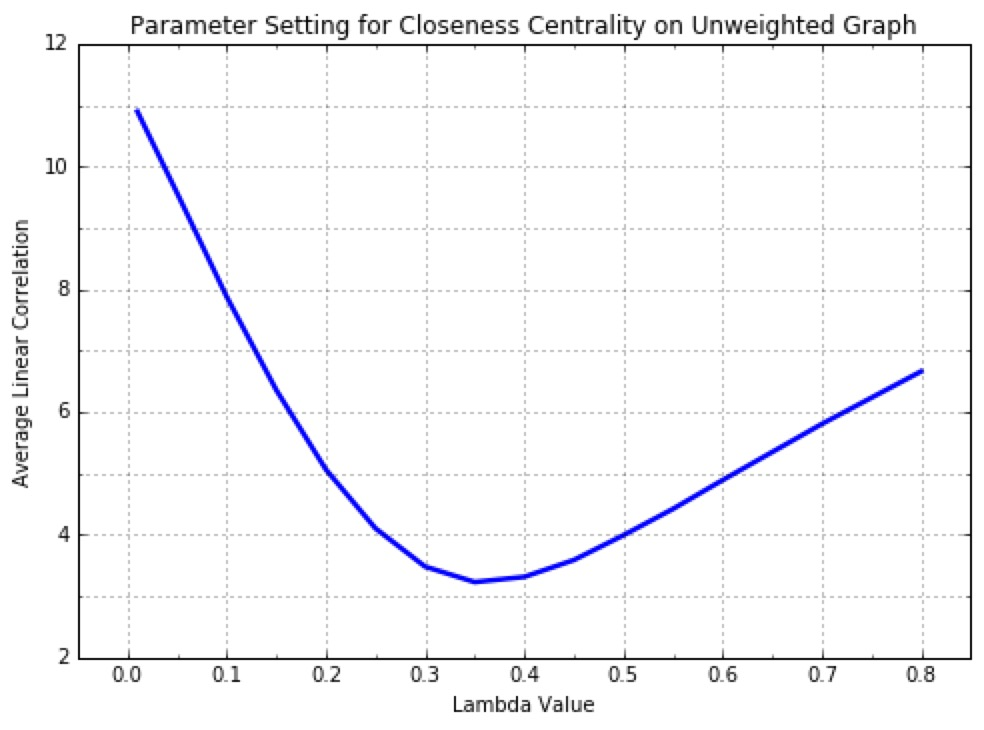
\includegraphics[scale = 0.2]{\main/img/CCU_2.jpeg}
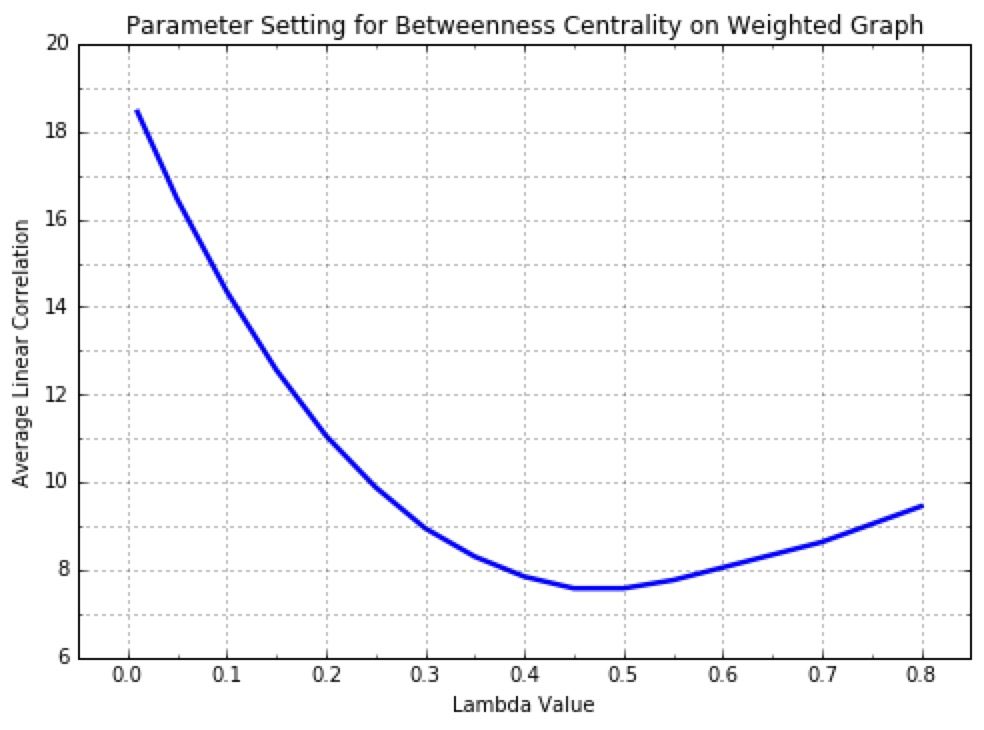
\includegraphics[scale = 0.2]{\main/img/BCW_2.jpeg}
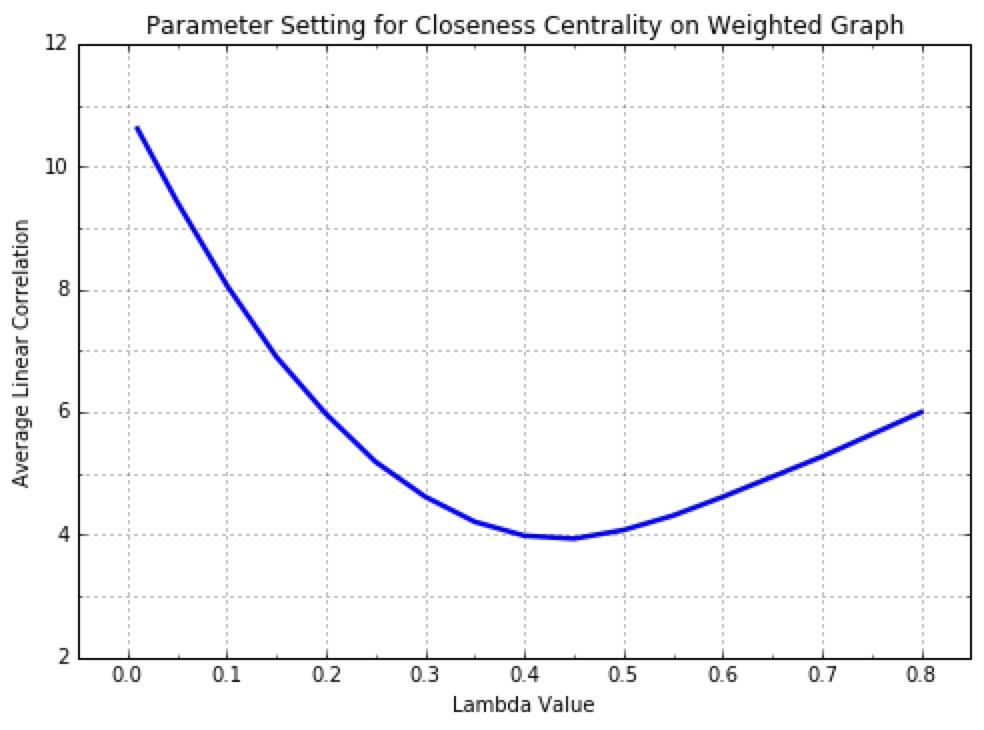
\includegraphics[scale = 0.2]{\main/img/CCW_2.jpeg}
\caption{Hyper-parameter validation}
\label{hyper}
\end{figure}

Each plot is obtained in the following way. First, we generated 20 probabilistic graphs and candidate $\lambda$ value, which ranges from 0.01 to 0.8; Next, on each probabilistic graph, we computed linear correlation strength under each $\lambda$, using our IPG method; Finally, we took the average linear correlation over 20 probabilistic graphs. From these four experiments we can conclude that the optimal choice of the hyper-parameter $\lambda$ varies with tasks, whereas all the optimal $\lambda's$ lie in the interval from 0.25 to 0.45. Though $\lambda=0.4$ is not always the optimal choice in different tasks, the results achieved by $\lambda=0.4$ is still competitive. Therefore, it is reasonable to choose $\lambda=0.4$.

\section{Conclusion}
In this Chapter, we provide a novel approach to deal with edge uncertainty in graph mining problems. Specifically, by taking the inverse of edge probability with a hyper-parameter, we can use existing existing centrality measures to rank entities. We empirically show the effectiveness of our IPG method by experiments. %First, by visualizing the centrality rankings in a dynamic network, we demonstrate IPG's ability to capture salient events underlying the evolution of network. Next, we compare the linear correlation of three method, Negative Logarithm, Most Probable Path, and Inversed Probabilistic Graphs, with sampling. Across a various of datasets and tasks, IPG has a steadily strong linear correlation with sampling compared to the other two. Finally, we compare the performance of the three methods in the previous example on a real dataset with ground truth. We assess the three methods by ROC curves, and results show that IPG still has advantages over NL and ML. 


\end{document}